%% FullCourse_10Lecs -- Lecture 4, Topic 4.1: Motivation + Optimal Growth Setup
%% Source: ./archive_pre_split/Lec04_DL_RL_Macro.tex (sections 1-2)

%% Shared preamble for the FullCourse_10Lecs topic decks.
%%
%% Each topic .tex \input's this file, then defines its own \title, \date
%% override (if any), \graphicspath, and \begin{document}.
%%
%% Reconstructed verbatim from the inlined copy preserved in
%% Lec10_Case_Studies/Lec10_T8_Case6_DeepRamsey.tex (lines 23-190), which is
%% explicitly annotated there as "from ../shared_preamble.tex, copied verbatim".
%% Base preamble matches MiniCourse_8hr/Slides/shared_preamble.tex; this version
%% additionally provides \sectiondivider, the conceptbox/cautionbox/examplebox/
%% takeawaybox tcolorboxes, and \compacttables used across the split decks.

\documentclass[10pt,english,aspectratio=169]{beamer}

\usepackage{ae,aecompl}
\usepackage[T1]{fontenc}
\usepackage{textcomp}
\usepackage[utf8]{inputenc}
\usepackage{babel}
\usepackage{datetime2}

\setcounter{secnumdepth}{3}
\setcounter{tocdepth}{3}

\usepackage{amsmath, amssymb, amsthm, graphicx}
\usepackage{booktabs, multirow}
\usepackage{tikz}
\usepackage{pgfplots}
\pgfplotsset{compat=1.16}
\usepackage[most]{tcolorbox}
\tcbuselibrary{skins, breakable, theorems}
\usepackage{listings}
\usepackage{xcolor}

\lstset{
  basicstyle=\ttfamily\small,
  keywordstyle=\color{blue!80!black}\bfseries,
  commentstyle=\color{green!50!black}\itshape,
  stringstyle=\color{orange!80!black},
  backgroundcolor=\color{gray!8},
  frame=single,
  rulecolor=\color{gray!40},
  breaklines=true,
  showstringspaces=false,
  numbers=none,
}

\lstdefinestyle{pythonstyle}{
    language=Python,
    basicstyle=\ttfamily\footnotesize,
    keywordstyle=\color{blue!80!black}\bfseries,
    commentstyle=\color{green!50!black}\itshape,
    stringstyle=\color{orange!80!black},
    frame=single,
    breaklines=true,
    showstringspaces=false,
    numbers=left,
    numbersep=5pt,
    numberstyle=\tiny\color{gray},
    backgroundcolor=\color{gray!8},
    rulecolor=\color{gray!40}
}

\ifx\hypersetup\undefined
  \AtBeginDocument{%
    \hypersetup{bookmarks=false,breaklinks=true,pdfborder={0 0 0},colorlinks=true,
      linkcolor=DarkText,urlcolor=RedTitle}%
  }
\else
  \hypersetup{bookmarks=false,breaklinks=true,pdfborder={0 0 0},colorlinks=true,
    linkcolor=DarkText,urlcolor=RedTitle}%
\fi

\makeatletter
\newcommand\makebeamertitle{%
  \begin{frame}[plain]
    \vspace*{1.0cm}
    \centering
    {\usebeamerfont{title}\usebeamercolor[fg]{title}\inserttitle\par}
    \vspace{1.0cm}
    {\usebeamerfont{author}\usebeamercolor[fg]{author}\insertauthor\par}
    \vspace{0.2cm}
    {\usebeamerfont{date}\usebeamercolor[fg]{date}\insertdate\par}
  \end{frame}}%
\AtBeginDocument{%
  \let\origtableofcontents=\tableofcontents
  \def\tableofcontents{\@ifnextchar[{\origtableofcontents}{\gobbletableofcontents}}
  \def\gobbletableofcontents#1{\origtableofcontents}%
}

\usetheme{metropolis}
\usefonttheme{professionalfonts}

\definecolor{LightGray}{RGB}{230,230,230}
\definecolor{RedTitle}{RGB}{0,0,200}
\definecolor{VeryLightGray}{RGB}{245,245,245}
\definecolor{DarkText}{RGB}{0,0,0}

\setbeamercolor{background canvas}{bg=white}
\setbeamercolor{title}{fg=RedTitle}
\setbeamercolor{author}{fg=DarkText}
\setbeamercolor{date}{fg=DarkText}
\setbeamercolor{frametitle}{bg=VeryLightGray,fg=DarkText}
\setbeamercolor{normal text}{fg=DarkText}
\setbeamerfont{title}{size=\large}

\setbeamersize{text margin left=5mm, text margin right=5mm}
\addtobeamertemplate{frametitle}{}{\vspace{-0.5em}}
\newcommand{\reducevspace}{\vspace{-0.5cm}}

% Shared section divider and box styles for split topic decks.
\newcommand{\sectiondivider}[2]{%
\begin{frame}[plain,noframenumbering]
\begin{center}
\vfill
{\Large\textbf{#1}\par}
\vspace{0.35cm}
{\normalsize #2\par}
\vfill
\end{center}
\end{frame}
}

\newtcolorbox{conceptbox}[1][]{
  colback=blue!3,
  colframe=RedTitle!55,
  boxrule=0.35mm,
  arc=1mm,
  left=2mm,
  right=2mm,
  top=1mm,
  bottom=1mm,
  #1
}
\newtcolorbox{cautionbox}[1][]{
  colback=red!3,
  colframe=red!50!black,
  boxrule=0.35mm,
  arc=1mm,
  left=2mm,
  right=2mm,
  top=1mm,
  bottom=1mm,
  #1
}
\newtcolorbox{examplebox}[1][]{
  colback=green!3,
  colframe=green!45!black,
  boxrule=0.35mm,
  arc=1mm,
  left=2mm,
  right=2mm,
  top=1mm,
  bottom=1mm,
  #1
}
\newtcolorbox{takeawaybox}[1][]{
  colback=VeryLightGray,
  colframe=RedTitle!55,
  boxrule=0.35mm,
  arc=1mm,
  left=2mm,
  right=2mm,
  top=1mm,
  bottom=1mm,
  #1
}
\newcommand{\compacttables}{\renewcommand{\arraystretch}{1.15}}

\setbeamertemplate{navigation symbols}{}
\setbeamertemplate{footline}{%
  \hfill%
  \usebeamercolor[fg]{page number in head/foot}%
  \usebeamerfont{page number in head/foot}%
  \insertframenumber\,/\,\inserttotalframenumber\kern1em\vskip2pt%
}

\makeatother

\author{Zhigang Feng}
% "date with time": compile timestamp so each build is identifiable.
\date{\today\ \DTMcurrenttime}


% The undergrad-foundations appendix must not inflate the main deck's
% "k/Total" footer: restart frame numbering at \appendix.
\usepackage{appendixnumberbeamer}

\graphicspath{{./pic/}{../../MiniCourse_8hr/Slides/Module2_DL_RL_Macro/pic/}{../}}

% Suppress the redundant auto-generated metropolis section page; the
% \sectiondivider frames below are the dividers we keep.
\metroset{sectionpage=none}
\usetikzlibrary{positioning,arrows.meta,shapes,calc}
%% Lec04 shared MAP slide: "one map, four acts" recurring diagram.
%% Input this file AFTER ../shared_preamble.tex (needs RedTitle, VeryLightGray,
%% DarkText) and AFTER \usetikzlibrary{positioning,arrows.meta,shapes,calc}.
%% Call \LecFourMap{k} inside a frame, where k in {1,2,3,4} highlights the
%% current act ("you are here") and k = 0 renders the closing reprise with all
%% four acts checked green (used by T4's closing frame).
%% Filename deliberately does NOT match the build glob Lec*_T*.tex, so the build
%% script never tries to compile it standalone.
%%
%% The four acts are the lecture's story: PROBLEM -> SOLVE -> CODE -> TRUST,
%% one running example throughout (the optimal growth model): why grids break,
%% the Bellman route (deep VFI + actor-critic), the Euler route in PyTorch,
%% and structured networks + the validation gate.

\newcommand{\LecFourMap}[1]{%
% Precompute per-box style selectors; TikZ option lists are comma-split before
% TeX conditionals run, so \ifnum must not sit inside a [...] options list.
\ifnum#1=0
  \tikzset{lmapa/.style={lmapdone}, lmapb/.style={lmapdone},
           lmapc/.style={lmapdone}, lmapd/.style={lmapdone}}%
\else
  \tikzset{lmapa/.style={}, lmapb/.style={}, lmapc/.style={}, lmapd/.style={}}%
  \ifnum#1=1 \tikzset{lmapa/.style={lmapcur}}\fi
  \ifnum#1=2 \tikzset{lmapb/.style={lmapcur}}\fi
  \ifnum#1=3 \tikzset{lmapc/.style={lmapcur}}\fi
  \ifnum#1=4 \tikzset{lmapd/.style={lmapcur}}\fi
\fi
\begin{center}
\begin{tikzpicture}[
    act/.style={rectangle, rounded corners, draw=black!60, fill=VeryLightGray,
        minimum width=3.0cm, minimum height=0.95cm, text width=2.9cm,
        align=center, font=\small, text=DarkText},
    lmapcur/.style={draw=RedTitle, very thick, fill=orange!20},
    lmapdone/.style={draw=green!45!black, thick, fill=green!10},
    q/.style={font=\tiny\itshape, text width=3.0cm, align=center, text=black!70},
    barlab/.style={font=\tiny\bfseries, text=black!65},
    sat/.style={rectangle, rounded corners, draw=black!45, dashed, fill=white,
        text width=5.2cm, align=center, font=\tiny, text=black!70,
        minimum height=0.5cm},
    arr/.style={-{Stealth[length=2.2mm]}, thick, gray!60}
]
    % --- four act boxes ---
    \node[act, lmapa] (a1) at (0,0)
        {\textbf{4.1\ \ PROBLEM}\\[1pt] \tiny growth model $\cdot$ curse of dim.};
    \node[act, lmapb] (a2) at (3.6,0)
        {\textbf{4.2\ \ SOLVE}\\[1pt] \tiny deep VFI $\cdot$ actor--critic};
    \node[act, lmapc] (a3) at (7.2,0)
        {\textbf{4.3\ \ CODE}\\[1pt] \tiny Euler loss $\cdot$ PyTorch};
    \node[act, lmapd] (a4) at (10.8,0)
        {\textbf{4.4\ \ TRUST}\\[1pt] \tiny ICNN $\cdot$ validation $\cdot$ lab};
    \draw[arr] (a1) -- (a2);
    \draw[arr] (a2) -- (a3);
    \draw[arr] (a3) -- (a4);
    % --- the student question each act answers ---
    \node[q] at (0,-0.95)    {why do grids break on\\ real macro models?};
    \node[q] at (3.6,-0.95)  {how do neural nets solve\\ the Bellman equation?};
    \node[q] at (7.2,-0.95)  {how do I code it --- loss,\\ networks, training loop?};
    \node[q] at (10.8,-0.95) {can I trust the answer ---\\ and how do I prove it?};
    % --- "you are here" marker above the current act ---
    \ifnum#1=1 \node[font=\scriptsize\bfseries, text=RedTitle] at (0,0.98)
        {you are here\ $\blacktriangledown$};\fi
    \ifnum#1=2 \node[font=\scriptsize\bfseries, text=RedTitle] at (3.6,0.98)
        {you are here\ $\blacktriangledown$};\fi
    \ifnum#1=3 \node[font=\scriptsize\bfseries, text=RedTitle] at (7.2,0.98)
        {you are here\ $\blacktriangledown$};\fi
    \ifnum#1=4 \node[font=\scriptsize\bfseries, text=RedTitle] at (10.8,0.98)
        {you are here\ $\blacktriangledown$};\fi
    \ifnum#1=0 \node[font=\scriptsize\bfseries, text=green!45!black] at (5.4,0.98)
        {all four acts complete};\fi
    % --- bottom band: two solution routes + the audit (the technical spine) ---
    \fill[blue!10]   (-1.55,-1.72) rectangle (5.15,-1.40);
    \fill[green!12]  (5.65,-1.72)  rectangle (8.75,-1.40);
    \fill[orange!16] (9.25,-1.72)  rectangle (12.35,-1.40);
    \node[barlab] at (1.8,-1.56)  {BELLMAN ROUTE\ ($V$, $g$ networks)};
    \node[barlab] at (7.2,-1.56)  {EULER ROUTE\ (FOC residuals)};
    \node[barlab] at (10.8,-1.56) {AUDIT GATE\ (Lab 3A/3B)};
    % --- dashed satellites: where this lecture sits in the course flow ---
    \node[sat] at (1.5,-2.42)
        {\textit{upstream:} Lec03 --- the NN toolkit (architecture, UAT, training, ICNN)};
    \node[sat] at (9.3,-2.42)
        {\textit{downstream:} Lec05 --- the RL theory behind actor--critic; Lec06 --- heterogeneous agents at scale};
\end{tikzpicture}
\end{center}
}


\title[AI for Econ Research]{AI for Economic Research: Dynamic Models, Language, and Agents\\
Lecture 4.1: Motivation \& the Optimal Growth Running Example}

\begin{document}

\makebeamertitle

%=============================================================================
\begin{frame}{Lecture 4 in One Map}
\textbf{One lecture, four decks, one running example: solve the optimal growth model with deep learning --- pose the problem, solve it two ways, code it, and prove the answer right.}

\LecFourMap{1}

\vspace{0.05cm}
\footnotesize\textit{\textbf{Act 4.1 (here)} poses the problem: the workhorse growth model and its Bellman equation, why grid methods hit the $N^d$ wall, and the closed-form benchmark plus grid VFI (Lab 3A) that will serve as ground truth for every neural method that follows.}
\end{frame}

%=============================================================================
\section{Motivation: Why Deep Learning for Macro Models?}

\sectiondivider{Motivation: Why Deep Learning for Macro Models?}{The workhorse growth model --- and the $N^d$ wall every grid method hits}

%---------------------------------------
\begin{frame}[label=mainWorkhorse]{The Workhorse: The Optimal Growth Model}
\textit{\footnotesize Nearly every quantitative macro model is a variation on one core structure --- the optimal (neoclassical) growth model.}
\hfill\hyperlink{appFoundations}{\beamergotobutton{\scriptsize New to dynamic macro? Appendix: Solow $\to$ Bellman}}

\vspace{0.05cm}
\begin{columns}
  \begin{column}{0.54\textwidth}
    \footnotesize
    \textbf{A planner maximizes lifetime welfare:}
    \[ \max_{\{c_t,\,k_{t+1}\}} \ \sum_{t=0}^\infty \beta^t\, u(c_t) \]
    \textbf{subject to the economy's resource constraint:}
    \[ c_t + k_{t+1} = \underbrace{f(k_t)+(1-\delta)k_t}_{\text{resources } y_t},\quad k_0\ \text{given} \]
    \textit{\scriptsize Cobb--Douglas output $f(k)=Ak^\alpha$; resources $=$ output $+$ undepreciated capital, split between consumption $c_t$ and next-period capital $k_{t+1}$.}
  \end{column}
  \begin{column}{0.46\textwidth}
    \footnotesize
    \textbf{Anatomy of the model:}
    \begin{conceptbox}
    \scriptsize
    \begin{tabular}{@{}p{1.7cm}@{\hspace{5pt}}l@{}}
      \textbf{Preferences} & concave $u$, discount $\beta\in(0,1)$ \\
      \textbf{Technology}  & $f(k)=Ak^\alpha$, deprec.\ $\delta$ \\
      \textbf{State}       & capital $k$ (inherited) \\
      \textbf{Control}     & saving $k'=g(k)$ \\
      \textbf{Solve for}   & value $V(k)$, policy $g(k)$ \\
    \end{tabular}
    \end{conceptbox}
    \medskip
    \textit{\scriptsize Two primitives --- tastes $(u,\beta)$ and technology $(f,\delta)$ --- plus one accounting identity generate the entire dynamic problem.}
  \end{column}
\end{columns}
\end{frame}

%---------------------------------------
\begin{frame}{The Workhorse: Recursive (Bellman) Formulation}
\textit{\footnotesize The infinite-horizon plan collapses to a one-step problem in a single state.}

\vspace{0.2cm}
\begin{itemize}
  \item \textbf{From sequence to recursion}: rather than choose the entire path $\{c_t,k_{t+1}\}_{t=0}^\infty$ at once, ask only --- given capital $k$ today, how much should we save?
  \medskip
  \item \textbf{Bellman equation} --- today's value $=$ current utility $+$ discounted continuation value:
    \[ V(k) = \max_{0\le k' \le y}\big\{\, u(y - k') + \beta\,V(k') \,\big\}, \qquad y = f(k)+(1-\delta)k \]
  \item The solution is a \emph{pair}: the value function $V(k)$ and the policy $k'=g(k)$. Consumption --- and, in market versions, prices --- follow from $g$.
  \medskip
  \item \textbf{A single state variable $k$} makes this cheap to solve on a grid --- and that very tractability is what breaks once the model grows richer.
\end{itemize}

\vspace{0.1cm}
{\footnotesize\textit{Running Example (Section 2) specializes this to the analytically solvable case ($A=1,\ \delta=1,\ u=\log$), giving the closed-form policy $c^*(y)=(1-\alpha\beta)\,y$ --- our ground truth for every neural method.}}
\end{frame}

%---------------------------------------
\begin{frame}{Why a Workhorse? One Model, Many Directions}
\begin{center}
\begin{tikzpicture}[scale=0.8, transform shape,
  trunk/.style={rectangle, rounded corners, draw=RedTitle!60, fill=RedTitle!12,
                align=center, minimum width=2.3cm, minimum height=1.5cm, font=\small\bfseries},
  br/.style={rectangle, rounded corners, draw=black!40, fill=VeryLightGray,
             align=left, text width=4.6cm, inner sep=3pt, font=\scriptsize},
  arr/.style={->, semithick, >=stealth, black!50}]
  \node[trunk] (m) at (0,0) {Optimal\\Growth\\Model};
  \node[font=\tiny, text=black!60] at (0,-1.2) {state: just $k$};
  \node[br] (b1) at (5.7, 3.0)  {\textcolor{orange!70!black}{\textbf{$+\,z$}}\ \ \textbf{Stochastic shocks}\\ \textcolor{black!55}{RBC $\Rightarrow$ business cycles}};
  \node[br] (b2) at (5.7, 1.5)  {\textcolor{orange!70!black}{\textbf{$+\,\mu$}}\ \ \textbf{Heterogeneous agents}\\ \textcolor{black!55}{Aiyagari, Krusell--Smith $\Rightarrow$ inequality}};
  \node[br] (b3) at (5.7, 0.0)  {\textcolor{orange!70!black}{\textbf{$+\,$age}}\ \ \textbf{Life-cycle / OLG}\\ \textcolor{black!55}{demographics, pensions}};
  \node[br] (b4) at (5.7, -1.5) {\textcolor{orange!70!black}{\textbf{$+\,$rigidities}}\ \ \textbf{Frictions}\\ \textcolor{black!55}{New Keynesian DSGE $\Rightarrow$ policy}};
  \node[br] (b5) at (5.7, -3.0) {\textcolor{orange!70!black}{\textbf{$+\,b$}}\ \ \textbf{Open economy}\\ \textcolor{black!55}{external debt, capital flows}};
  \draw[arr] (m.east) to[out=25,in=180]  (b1.west);
  \draw[arr] (m.east) to[out=13,in=180]  (b2.west);
  \draw[arr] (m.east) --                 (b3.west);
  \draw[arr] (m.east) to[out=-13,in=180] (b4.west);
  \draw[arr] (m.east) to[out=-25,in=180] (b5.west);
\end{tikzpicture}
\end{center}
\vspace{-0.1cm}
\begin{takeawaybox}
\footnotesize
\textbf{Same skeleton, richer flesh} --- the trunk is the optimal growth model, each realistic direction a branch (cf.\ the extensions map in Lecture 1). Master the trunk once and every branch is within reach --- but \emph{each branch adds state variables}, and more state means ``harder to compute.''
\end{takeawaybox}
\end{frame}

%---------------------------------------
\begin{frame}{The Catch: Every Direction Adds State Variables}
\begin{itemize}
  \item Each realistic ingredient enlarges the \textbf{state vector} the solution must carry:
\end{itemize}
\vspace{0.15cm}
\begin{center}
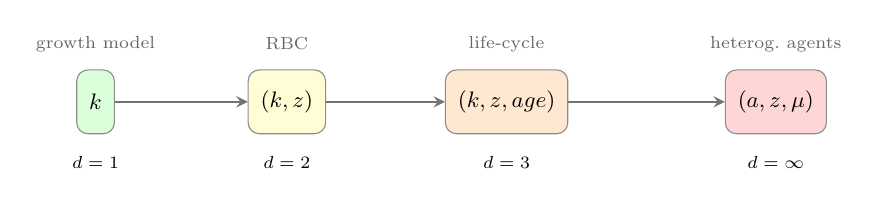
\begin{tikzpicture}[scale=0.9, transform shape,
  sbox/.style={rectangle, rounded corners, draw=black!45, align=center,
               minimum height=0.9cm, inner sep=5pt, font=\small},
  arr/.style={->, thick, >=stealth, black!55}]
  \node[sbox, fill=green!14]  (s1) at (0,0)   {$k$};
  \node[sbox, fill=yellow!16] (s2) at (2.7,0) {$(k,z)$};
  \node[sbox, fill=orange!18] (s3) at (5.8,0) {$(k,z,\text{age})$};
  \node[sbox, fill=red!16]    (s4) at (9.6,0) {$(a,z,\mu)$};
  \draw[arr] (s1)--(s2); \draw[arr] (s2)--(s3); \draw[arr] (s3)--(s4);
  \node[font=\scriptsize] at (0,-0.85)   {$d=1$};
  \node[font=\scriptsize] at (2.7,-0.85) {$d=2$};
  \node[font=\scriptsize] at (5.8,-0.85) {$d=3$};
  \node[font=\scriptsize] at (9.6,-0.85) {$d=\infty$};
  \node[font=\scriptsize, text=black!60] at (0,0.82)   {growth model};
  \node[font=\scriptsize, text=black!60] at (2.7,0.82) {RBC};
  \node[font=\scriptsize, text=black!60] at (5.8,0.82) {life-cycle};
  \node[font=\scriptsize, text=black!60] at (9.6,0.82) {heterog.\ agents};
\end{tikzpicture}
\end{center}
\vspace{0.1cm}
\begin{itemize}
  \item A grid needs $N^d$ points --- cost \textbf{explodes} with every added dimension (Bellman's \emph{curse of dimensionality}).
  \item The workhorse is trivial at $d=1$; its research-frontier descendants quickly reach $d\ge 10$ --- or carry a whole \emph{distribution} $\mu$ (infinite-dimensional).
  \item \textbf{This is the wall.} The rest of Topic 4.1 asks: can \emph{deep learning} scale where grids cannot?
\end{itemize}
\end{frame}

%---------------------------------------
\begin{frame}{The Computational Frontier in Macro}
\begin{itemize}
  \item Quantitative macroeconomics solves dynamic optimization problems:
    \[
      V(k) = \max_{k'} \Big\{ u\big(f(k) - k'\big) + \beta\, V(k') \Big\}
    \]
  \item \textbf{Standard toolkit}: Value Function Iteration (VFI), Euler equation methods, perturbation
  \medskip
  \item These methods have served the profession well for decades
  \item But they face fundamental limitations as models grow richer:
    \begin{itemize}
      \item More state variables (capital, bonds, housing, human capital\ldots)
      \item Heterogeneous agents (wealth distributions, idiosyncratic risk)
      \item Aggregate uncertainty (business cycles in HA models)
    \end{itemize}
  \medskip
  \item \textbf{This lecture}: How deep learning and reinforcement learning offer a fundamentally different approach
\end{itemize}

\vspace{0.15cm}
{\footnotesize\textit{Course arc: Lec02 T2 framed AI as \textbf{cognitive capital} (the \emph{why}); Lec03 delivered NN architectures and training algorithms (the \emph{what}); Lec04 closes the loop --- turning those tools on the optimal-growth Bellman equation (the \emph{how}).}}
\end{frame}

%---------------------------------------
\begin{frame}{The Naive Approach: Grid-Based Methods}
\begin{itemize}
  \item \textbf{Value Function Iteration on a grid}:
    \begin{enumerate}
      \item Discretize the state space: $\{k_1, k_2, \ldots, k_N\}$
      \item For each grid point, solve $\max_{k'} \{u(f(k_i) - k') + \beta V(k')\}$
      \item Iterate until convergence
    \end{enumerate}
  \medskip
  \item \textbf{This works well} when:
    \begin{itemize}
      \item The state space is low-dimensional (1--3 variables)
      \item The functions are smooth
      \item We can afford to evaluate $V$ at every grid point
    \end{itemize}
  \medskip
  \item Alternatives like Chebyshev polynomials and finite elements improve efficiency but share the same fundamental scaling problem
\end{itemize}
\end{frame}

%---------------------------------------
\begin{frame}{The Curse of Dimensionality: The $N^d$ Explosion}
\begin{columns}
  \begin{column}{0.52\textwidth}
    \footnotesize
    A grid places $N$ points \emph{per dimension}, so covering $d$ dimensions costs $N^d$ points. With $N = 100$:
    \begin{itemize}\footnotesize
      \item $d = 1$: \ $10^{2}$ pts \quad (trivial)
      \item $d = 2$: \ $10^{4}$ pts \quad (manageable)
      \item $d = 5$: \ $10^{10}$ pts \quad (infeasible)
      \item $d = 10$: $10^{20}$ pts \quad (absurd)
    \end{itemize}
    \medskip
    \textbf{Linear in dimension, but exponential in resolution} --- every extra state variable multiplies the cost by another factor of $N$.
  \end{column}
  \begin{column}{0.48\textwidth}
    \centering
    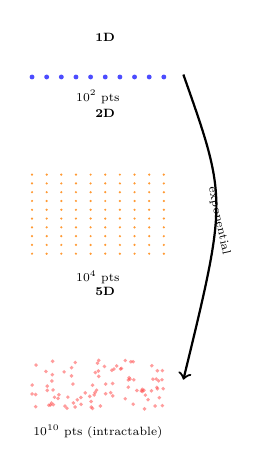
\begin{tikzpicture}[scale=0.62, transform shape, every node/.style={font=\scriptsize}]
      % 1D: 10 dots on a line
      \node[anchor=south] at (1.5, 0.6) {\textbf{1D}};
      \foreach \x in {0,1,...,9} {
        \fill[blue!70] (\x*0.3, 0) circle (0.05);
      }
      \node[anchor=north] at (1.35, -0.15) {$10^{2}$ pts};

      % 2D: 10x10 grid
      \node[anchor=south] at (1.5, -0.95) {\textbf{2D}};
      \foreach \x in {0,1,...,9}{
        \foreach \y in {0,1,...,9}{
          \fill[orange!80] (\x*0.3, -2 - \y*0.18) circle (0.025);
        }
      }
      \node[anchor=north] at (1.35, -3.85) {$10^{4}$ pts};

      % 5D: cloud (intractable)
      \node[anchor=south] at (1.5, -4.6) {\textbf{5D}};
      \foreach \i in {1,...,90}{
        \pgfmathsetmacro{\rx}{rnd*2.7}
        \pgfmathsetmacro{\ry}{rnd*1.0}
        \fill[red!70,opacity=0.55] (\rx, -5.8 - \ry) circle (0.04);
      }
      \node[anchor=north] at (1.35, -7.0) {$10^{10}$ pts (intractable)};

      \draw[->,thick] (3.1, 0.05) .. controls (4.0, -2.5) .. (3.1, -6.2);
      \node[rotate=-78,anchor=south] at (3.6,-3.0) {\scriptsize exponential};
    \end{tikzpicture}
    \vspace{-0.1cm}
    \footnotesize\textit{Dots are a schematic sample, not the literal count ($N=100$ per axis).}
  \end{column}
\end{columns}
\end{frame}

%---------------------------------------
\begin{frame}{Why Grids Break: Real Macro Models Are High-Dimensional}
\begin{itemize}
  \item \textbf{Real macro models} routinely have $d \geq 10$ --- and often far more:
    \begin{itemize}\footnotesize
      \item Krusell \& Smith (1998), JPE: individual $k$ $+$ aggregate $K$ $+$ shocks
      \item Life-cycle: age $+$ assets $+$ earnings $+$ health $+ \cdots$
      \item HA $+$ aggregate risk: the \emph{whole} wealth distribution (infinite-dimensional)
    \end{itemize}
  \medskip
  \item \textit{Canonical HA benchmarks:} Aiyagari (1994), QJE; Krusell \& Smith (1998), JPE.
  \item These are the curse-of-dimensionality test cases \textbf{Lec06} attacks with DL/RL methods; \textbf{Lec09} reuses Aiyagari as its running example.
  \medskip
  \item \textbf{Grid-based methods cannot scale to these problems} --- at $10^{20}$ points, no amount of hardware helps.
\end{itemize}
\end{frame}

%---------------------------------------
\begin{frame}{Beyond Grids: Other Classical Limitations}
\begin{itemize}
  \item \textbf{Perturbation methods} (linearization around steady state):
    \begin{itemize}
      \item Fast and accurate locally
      \item But may lose accuracy far from steady state
      \item Struggle with non-linearities, occasionally binding constraints, regime switches
    \end{itemize}
  \medskip
  \item \textbf{Projection methods} (Chebyshev, finite elements):
    \begin{itemize}
      \item Globally accurate for smooth problems
      \item Require structured grids or node sets
      \item Still suffer from the curse of dimensionality
    \end{itemize}
  \medskip
  \item \textbf{Kinks and non-convexities}:
    \begin{itemize}
      \item Borrowing constraints, irreversible investment, discrete choices
      \item First-order conditions fail or require complex root-finding
    \end{itemize}
  \medskip
  \item We need function approximators that scale gracefully with dimension and handle irregular structures
\end{itemize}
\end{frame}

%---------------------------------------
\begin{frame}{The Deep Learning Opportunity: Approximation That Scales}
\begin{itemize}
  \item \textbf{Neural networks are universal function approximators}:
    \begin{itemize}
      \item With enough hidden units, a network can represent \emph{any} continuous function on a compact set (Cybenko 1989; Hornik et al.\ 1989).
    \end{itemize}
  \medskip
  \item \textbf{And they scale with dimension}:
    \begin{itemize}
      \item Parameter count grows \emph{polynomially} with the input dimension, not exponentially (Barron 1993).
      \item A grid needs $N^d$ points; a network needs a weight count that grows gently with $d$.
    \end{itemize}
  \medskip
  \item \textbf{So represent the value or policy function as a network} --- $V_\theta(k)$ or $g_\theta(k)$ --- and \emph{learn} the weights $\theta$; there is no grid to discretize.
  \medskip
  \item This is the escape from the curse of dimensionality: replace ``store a value at every grid point'' with ``fit one smooth function that generalizes.''
\end{itemize}
\end{frame}

%---------------------------------------
\begin{frame}{The Deep Learning Opportunity: Differentiation \& Hardware}
\begin{itemize}
  \item \textbf{Automatic differentiation gives gradients for free}: Euler equations, FOCs, and Jacobians are differentiated straight from the code (PyTorch) --- no hand-derived, hand-coded derivatives.
  \medskip
  \item \textbf{Why GPUs accelerate deep learning}:
    \begin{itemize}\footnotesize
      \item A network's forward and backward passes are \emph{dense matrix multiplications} ($Wx$); training repeats billions of multiply--adds.
      \item A GPU packs \emph{thousands} of arithmetic cores (a CPU has a handful) that apply one operation to many numbers at once (SIMD), fed by very high memory bandwidth --- exactly what matrix multiplication needs.
      \item The work is \emph{parallel across the batch}: thousands of sampled states $(k,z)$, or a whole panel of simulated agents, run at once --- so one gradient step over thousands of states costs about what a CPU spends on a handful.
    \end{itemize}
  \medskip
  \item \textbf{The key insight}: recast the macro model as a \emph{learning problem} --- the policy or value function is the object to be learned, trained by stochastic gradient descent on sampled states.
\end{itemize}
\end{frame}

%---------------------------------------
\begin{frame}{The Inspiration: AlphaGo and Economic Models}
\textit{\footnotesize Silver et al.\ (2016, Nature), ``Mastering the Game of Go with Deep Neural Networks and Tree Search.''}
\begin{columns}
  \begin{column}{0.52\textwidth}
    \footnotesize
    \begin{itemize}
      \item \textbf{AlphaGo} (DeepMind, 2016) solved a problem with $\sim 10^{170}$ board states.
      \item It did \emph{not} enumerate the state space or solve the full Bellman equation on a grid.
      \item \textbf{It used two neural networks}:
        \begin{itemize}\footnotesize
          \item \textbf{Policy Net (Actor)}: ``Intuition'' --- which move to play.
          \item \textbf{Value Net (Critic)}: ``Judgment'' --- who is winning.
        \end{itemize}
      \item \textbf{Lesson for economics}: when the state space is too vast (e.g., wealth distribution in a HA model), use the same two-network approach.
      \item \textbf{This lecture}: apply the actor-critic idea to the optimal growth model as a proof of concept, then discuss scaling.
    \end{itemize}
  \end{column}
  \begin{column}{0.48\textwidth}
    \centering
    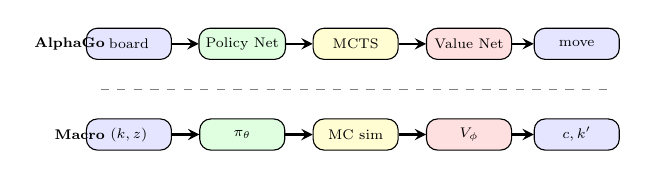
\begin{tikzpicture}[scale=0.72, transform shape,
      box/.style={rectangle,draw,rounded corners,minimum width=1.5cm,minimum height=0.55cm,align=center,font=\scriptsize},
      arr/.style={->,thick,>=stealth,font=\tiny}
    ]
      % AlphaGo row
      \node[box,fill=blue!10] (b) at (0,2)   {board};
      \node[box,fill=green!12] (pn) at (2,2) {Policy Net};
      \node[box,fill=yellow!18] (mc) at (4,2) {MCTS};
      \node[box,fill=red!12] (vn) at (6,2)   {Value Net};
      \node[box,fill=blue!10] (mv) at (7.9,2) {move};
      \draw[arr] (b) -- (pn); \draw[arr] (pn) -- (mc); \draw[arr] (mc) -- (vn); \draw[arr] (vn) -- (mv);
      \node[anchor=east,font=\scriptsize] at (-0.3,2) {\textbf{AlphaGo}};

      % Macro row
      \node[box,fill=blue!10] (s) at (0,0.4)    {$(k,z)$};
      \node[box,fill=green!12] (pi) at (2,0.4)  {$\pi_\theta$};
      \node[box,fill=yellow!18] (sim) at (4,0.4){MC sim};
      \node[box,fill=red!12] (vphi) at (6,0.4)  {$V_\phi$};
      \node[box,fill=blue!10] (c) at (7.9,0.4)  {$c, k'$};
      \draw[arr] (s) -- (pi); \draw[arr] (pi) -- (sim); \draw[arr] (sim) -- (vphi); \draw[arr] (vphi) -- (c);
      \node[anchor=east,font=\scriptsize] at (-0.3,0.4) {\textbf{Macro}};

      \draw[dashed,gray] (-0.5,1.2) -- (8.5,1.2);
    \end{tikzpicture}

    \vspace{0.05cm}
    {\scriptsize\textit{Same architectural pattern; different state space.}}
  \end{column}
\end{columns}
\end{frame}

%---------------------------------------
\begin{frame}{Reframing Macro as a Machine Learning Problem}
\begin{itemize}
  \item The optimal growth model can be recast as a \textbf{learning problem}:
    \begin{itemize}
      \item The decision rule $g(k)$ is approximated by a neural network
      \item The first-order conditions provide a natural \textbf{loss function}
      \item Modern optimization (Adam, SGD) and automatic differentiation drive training
    \end{itemize}
  \medskip
  \item \textbf{Two complementary approaches}:
    \begin{enumerate}
      \item \textbf{Deep Value Function Iteration}: Train networks to satisfy the Bellman equation (reinforcement learning flavor)
      \item \textbf{Euler Equation Minimization}: Train a network to satisfy the FOCs (supervised learning flavor)
    \end{enumerate}
  \medskip
  \item Both use the same building blocks:
    \begin{itemize}
      \item Neural network function approximation
      \item Stochastic gradient descent
      \item Monte Carlo sampling of state space
    \end{itemize}
\end{itemize}
\end{frame}

%=============================================================================
\section{Running Example: The Optimal Growth Model}

\sectiondivider{Running Example: The Optimal Growth Model}{A closed-form benchmark and grid VFI: the ground truth the networks must beat}

%---------------------------------------
\begin{frame}{Optimal Growth Model: Setup}
\textit{\footnotesize Recall the workhorse from Section 1 --- here we pin down the analytically solvable special case.}

\medskip
\begin{itemize}
  \item \textbf{Objective}: Maximize discounted lifetime utility:
    \[
      \max_{\{k_{t+1}\}} \sum_{t=0}^{\infty} \beta^t u\Big(f(k_t) - k_{t+1}\Big)
    \]
  \item \textbf{Production function}: $f(k_t) = k_t^\alpha$
  \item \textbf{Resource constraint}: Consumption $c_t = f(k_t) - k_{t+1}$
  \item \textbf{Depreciation}: $\delta = 1$ (full depreciation) in our benchmark; adjustable for general cases
  \medskip
  \item \textbf{Steady-state capital}:
    \[
      k_{ss} = \left(\frac{1}{\alpha\beta}\right)^{\frac{1}{\alpha - 1}} = (\alpha\beta)^{\frac{1}{1-\alpha}}
    \]
  \medskip
  \item \textbf{Why this model?} Simple enough for an analytical solution (ground truth), yet contains all the essential structure of richer models
\end{itemize}
\end{frame}

%---------------------------------------
\begin{frame}[label=mainVFI]{Bellman Equation and VFI}
\begin{itemize}
  \item \textbf{Recursive formulation} (Bellman equation):
    \[
      V(k) = \max_{k'} \Big\{ u\big(f(k) - k'\big) + \beta\, V(k') \Big\}
    \]
  \item \textbf{Value Function Iteration}:
    \begin{enumerate}
      \item Start with initial guess $V^0(k)$
      \item Update: $V^{n+1}(k) = \max_{k'}\{u(f(k) - k') + \beta\, V^n(k')\}$
      \item Repeat until $\|V^{n+1} - V^n\| < \text{tolerance}$
    \end{enumerate}
  \medskip
  \item \textbf{Contraction Mapping Theorem (Banach)}: Under standard assumptions, the Bellman operator $T$ is a contraction with modulus $\beta$
    \begin{itemize}
      \item Guarantees convergence to a unique fixed point $V^*$
      \item VFI converges \emph{geometrically} at rate $\beta$
      \item This is the theoretical foundation we build on
    \end{itemize}
\end{itemize}

\vspace{0.05cm}
\hfill\hyperlink{appCMT}{\beamergotobutton{\scriptsize Full statements: CMT $+$ Blackwell (Appendix)}}
\end{frame}

%---------------------------------------
\begin{frame}{Stochastic Extension}
\begin{itemize}
  \item Add a productivity shock $z$:
    \[
      v(y) = \max_{0 \leq c \leq y} \Big\{ u(c) + \beta\, \mathbb{E}\big[v(y')\big] \Big\}
    \]
  \item Transition: $y' = f(y - c)\cdot z$, where $z$ is i.i.d.\ log-normal
  \medskip
  \item \textbf{Analytical solution} for log utility $u(c) = \ln(c)$ and Cobb-Douglas $f(k) = k^\alpha$:
    \begin{align*}
      V^*(y) &= A + B \ln y \quad \text{(value function)} \\
      c^*(y) &= (1 - \alpha\beta)\, y \quad \text{(optimal policy: consume fixed fraction)}
    \end{align*}
  \medskip
  \item This closed-form solution serves as our \textbf{ground truth} for validating all neural network methods
  \item Lab 3A builds this benchmark via classical VFI with interpolation
\end{itemize}
\end{frame}

%---------------------------------------
\begin{frame}{VFI with Interpolation: The Classical Algorithm}
\begin{itemize}
  \item Since $y$ is continuous, we use interpolation on a grid:
  \medskip
  \begin{enumerate}
    \item \textbf{Initialize}: Grid $\{y_1, \ldots, y_N\}$, initial guess $v^0$
    \item \textbf{Interpolate}: Create function $\hat{v}(y)$ connecting $(y_i, v^0_i)$ pairs
    \item \textbf{Bellman update}: For each $y_i$:
      \[
        v^{\text{new}}_i = \max_c \left\{\ln(c) + \beta \sum_j \hat{v}\big(f(y_i - c)\, z_j\big)\, \phi(z_j)\right\}
      \]
    \item \textbf{Check convergence}: If $\|v^{\text{new}} - v^0\| < \text{tol}$, stop; else repeat
  \end{enumerate}
  \medskip
  \item This is the \textbf{benchmark} algorithm implemented in Lab 3A
  \item Works beautifully for 1D\ldots but the grid makes it impractical for higher dimensions
\end{itemize}
\end{frame}

%=============================================================================
% House-style bridge closer (matches Lec05/Lec09): restate the act, hand off.
\begin{frame}{Bridge: The Problem Is Set --- Now Replace the Grid}
\textbf{Act 4.1 posed the problem. The optimal growth model is the workhorse of quantitative macro, its Bellman equation is the object every solver must satisfy --- and grid-based VFI, exact in one dimension, collapses under the $N^d$ explosion.}

\vspace{0.25cm}
\begin{itemize}
  \item You now hold the benchmark: a closed-form special case and grid VFI (Lab 3A) --- the ground truth every neural solution in this lecture must reproduce.
  \item \textbf{Next (4.2):} swap the grid for parameters --- approximate $V$ and $g$ with neural networks and train them on the Bellman equation itself, actor--critic style.
\end{itemize}

\vspace{0.3cm}
\begin{center}
\footnotesize\textit{Arc: \textbf{4.1 PROBLEM} (growth model $+$ curse) $\;\to\;$ 4.2 SOLVE (deep VFI $+$ actor--critic) $\;\to\;$ 4.3 CODE (Euler $+$ PyTorch) $\;\to\;$ 4.4 TRUST (structure $+$ validation).}
\end{center}
\end{frame}

%=============================================================================
%  APPENDIX --- Dynamic Macro Foundations (undergraduate refresher)
%  Self-contained build-up from the Solow model to the recursive toolkit,
%  for audiences meeting dynamic macro for the first time. Entry buttons sit
%  on the "Workhorse" frame (label mainWorkhorse) and the "Bellman Equation
%  and VFI" frame (label mainVFI); every appendix frame returns to the former.
%  Navigation markup follows Lec10_T8_Case6_DeepRamsey_paper.tex.
%=============================================================================
\appendix
% Metropolis's \appendix hook swaps back its own plain footline with
% numbering=none, silently erasing the shared-preamble "k/Total" footer.
% Re-assert the house footline so appendix pages number as 1/12 ... 12/12
% (appendix-local, courtesy of appendixnumberbeamer).
\setbeamertemplate{footline}{%
  \hfill%
  \usebeamercolor[fg]{page number in head/foot}%
  \usebeamerfont{page number in head/foot}%
  \insertframenumber\,/\,\inserttotalframenumber\kern1em\vskip2pt%
}

\sectiondivider{Appendix: Dynamic Macro Foundations}{From Solow to Bellman --- a self-contained refresher, no dynamic macro assumed\\ (statements and intuition only; proofs live in your macro-theory course)}

%---------------------------------------
\begin{frame}[label=appFoundations]{Appendix Roadmap: From Solow to Bellman}
\textit{\footnotesize Everything the lecture takes for granted, built in eleven short steps --- click any step to jump; the arrow button on every page returns to the lecture.}
\hfill\hyperlink{mainWorkhorse}{\beamerreturnbutton{\scriptsize Return to lecture}}

\vspace{0.05cm}
\begin{center}
\begin{tikzpicture}[
  astep/.style={rectangle, rounded corners, draw=black!50, fill=VeryLightGray,
               minimum width=3.0cm, text width=2.9cm, minimum height=0.74cm,
               align=center, inner sep=2pt},
  grp/.style={font=\tiny\bfseries, text=RedTitle, anchor=west},
  arr/.style={->, >=stealth, semithick, black!55}]
  % --- Row 1: build the model ---
  \node[grp] at (-1.5,2.62) {BUILD THE MODEL};
  \node[astep] (s1) at (0,1.9)
    {\scriptsize\hyperlink{appSolow}{\textbf{A1\ \ Solow}}\\[-1pt] \tiny growth without choices};
  \node[astep] (s2) at (3.6,1.9)
    {\scriptsize\hyperlink{appRamsey}{\textbf{A2\ \ Add preferences}}\\[-1pt] \tiny saving becomes a choice};
  \node[astep] (s3) at (7.2,1.9)
    {\scriptsize\hyperlink{appSeqProblem}{\textbf{A3\ \ Sequential problem}}\\[-1pt] \tiny choose an infinite path};
  \node[astep] (s4) at (10.8,1.9)
    {\scriptsize\hyperlink{appMarkov}{\textbf{A4\ \ Markov structure}}\\[-1pt] \tiny the state $(k,z)$};
  \draw[arr] (s1) -- (s2); \draw[arr] (s2) -- (s3); \draw[arr] (s3) -- (s4);
  % --- Row 2: two formulations, one problem ---
  \node[grp] at (-1.5,0.72) {TWO FORMULATIONS, ONE PROBLEM};
  \node[astep] (s5) at (0,0)
    {\scriptsize\hyperlink{appBellman}{\textbf{A5\ \ Bellman equation}}\\[-1pt] \tiny recursion $+$ intuition};
  \node[astep] (s6) at (3.6,0)
    {\scriptsize\hyperlink{appEquivalence}{\textbf{A6\ \ Equivalence}}\\[-1pt] \tiny the four questions};
  \node[astep] (s7) at (7.2,0)
    {\scriptsize\hyperlink{appFunction}{\textbf{A7\ \ One function}}\\[-1pt] \tiny ``finite''-dimensional};
  \draw[arr, rounded corners=3pt] (s4.south) -- (10.8,0.95) -- (0,0.95) -- (s5.north);
  \draw[arr] (s5) -- (s6); \draw[arr] (s6) -- (s7);
  % --- Row 3: why it all works ---
  \node[grp] at (-1.5,-1.18) {WHY IT ALL WORKS};
  \node[astep] (s8) at (0,-1.9)
    {\scriptsize\hyperlink{appCMT}{\textbf{A8\ \ Contraction}}\\[-1pt] \tiny VFI must converge};
  \node[astep] (s9) at (3.6,-1.9)
    {\scriptsize\hyperlink{appBlackwell}{\textbf{A9\ \ Blackwell}}\\[-1pt] \tiny two easy conditions};
  \node[astep] (s10) at (7.2,-1.9)
    {\scriptsize\hyperlink{appBerge}{\textbf{A10\ \ Nice properties}}\\[-1pt] \tiny continuity, concavity};
  \node[astep] (s11) at (10.8,-1.9)
    {\scriptsize\hyperlink{appSummary}{\textbf{A11\ \ Summary}}\\[-1pt] \tiny $+$ where to learn more};
  \draw[arr, rounded corners=3pt] (s7.south) -- (7.2,-0.95) -- (0,-0.95) -- (s8.north);
  \draw[arr] (s8) -- (s9); \draw[arr] (s9) -- (s10); \draw[arr] (s10) -- (s11);
\end{tikzpicture}
\end{center}
\end{frame}

%---------------------------------------
\begin{frame}[label=appSolow]{Appendix A1 --- Where It All Starts: The Solow Growth Model}
\textit{\footnotesize The one dynamic model every undergraduate meets --- capital accumulation with a rule-of-thumb saver.}
\hfill\hyperlink{mainWorkhorse}{\beamerreturnbutton{\scriptsize Return to lecture}}

\vspace{0.1cm}
\begin{columns}
  \begin{column}{0.56\textwidth}
    \footnotesize
    \textbf{Technology} (per-worker terms): output from capital,
    $y_t = f(k_t) = A k_t^{\alpha}$, $\alpha\in(0,1)$ (diminishing returns).

    \smallskip
    \textbf{Behavior --- one assumed number}: save a \emph{fixed} fraction $s$ of output: $i_t = s\,y_t$, consume the rest, $c_t=(1-s)\,y_t$.

    \smallskip
    \textbf{The engine} --- capital accumulation:
    \[ k_{t+1} = (1-\delta)\,k_t + s A k_t^{\alpha} \]

    \textbf{Steady state} (saving $=$ replacement):
    $\;sAk^{*\alpha} = \delta k^{*} \Rightarrow k^{*} = \left(sA/\delta\right)^{\frac{1}{1-\alpha}}$; concavity makes it unique, with monotone convergence from any $k_0>0$.
  \end{column}
  \begin{column}{0.44\textwidth}
    \centering
    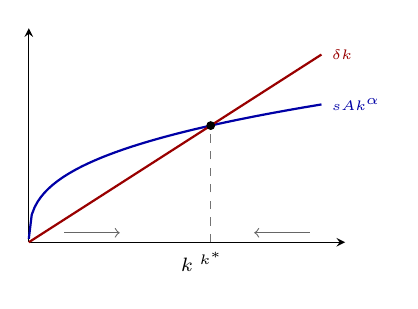
\begin{tikzpicture}
    \begin{axis}[width=5.6cm, height=4.3cm,
      axis lines=left, xlabel={\scriptsize $k$},
      xtick=\empty, ytick=\empty, xmin=0, xmax=4.0, ymin=0, ymax=1.35,
      clip=false, every axis plot/.append style={thick}]
      \addplot[domain=0.0001:3.7, samples=100, blue!65!black] {0.55*x^0.35}
        node[pos=1, right, font=\tiny, text=blue!65!black] {$sAk^{\alpha}$};
      \addplot[domain=0:3.7, red!60!black] {0.32*x}
        node[pos=1, right, font=\tiny, text=red!60!black] {$\delta k$};
      \draw[dashed, black!55] (axis cs:2.30,0) -- (axis cs:2.30,0.736);
      \fill (axis cs:2.30,0.736) circle[radius=1.6pt];
      \node[below, font=\tiny] at (axis cs:2.30,0) {$k^{*}$};
      \draw[->, black!60] (axis cs:0.45,0.06) -- (axis cs:1.15,0.06);
      \draw[->, black!60] (axis cs:3.55,0.06) -- (axis cs:2.85,0.06);
    \end{axis}
    \end{tikzpicture}

    \vspace{0.02cm}
    \tiny\textit{Below $k^{*}$ saving exceeds replacement, so $k$ grows; above, it shrinks --- the arrows on the axis.}
  \end{column}
\end{columns}
\vspace{0.05cm}
\begin{takeawaybox}
\footnotesize \textbf{Growth without choices.} Given $s$, the dynamics are fully mechanical --- nobody in the model ever decides anything. Solow (1956, \emph{QJE}) explains capital accumulation but stays silent on welfare: is $s$ a \emph{good} saving rate?
\end{takeawaybox}
\end{frame}

%---------------------------------------
\begin{frame}[label=appRamsey]{Appendix A2 --- From Solow to Optimal Growth: Make Saving a Choice}
\textit{\footnotesize Same technology, new question: instead of assuming how much society saves, derive it from preferences.}
\hfill\hyperlink{mainWorkhorse}{\beamerreturnbutton{\scriptsize Return to lecture}}

\begin{itemize}\footnotesize
  \item \textbf{What Solow cannot answer:} Is $s$ too high or too low for welfare? Would it respond to a capital-income tax? A ``golden-rule'' $s$ exists --- but nothing makes households pick it.
  \item \textbf{The upgrade --- keep the technology, add preferences:} technology stays Solow's ($f(k)=Ak^{\alpha}$, depreciation $\delta$); households now rank consumption streams $\;\mathbb{E}_0\sum_{t=0}^{\infty}\beta^t u(c_t)$, with $u'>0$, $u''<0$ (the smoothing motive) and $\beta\in(0,1)$ (impatience).
  \item Each period, resources are \emph{chosen} between $c_t$ (utility now) and $k_{t+1}$ (resources tomorrow) --- the intertemporal trade-off.
  \item \textbf{The saving rate becomes an outcome} --- endogenous, generally time-varying --- and the model becomes the \emph{optimal growth model} of this deck's opening slides. Planner $=$ competitive equilibrium here (welfare theorems), so the planner's problem is without loss.
\end{itemize}

\begin{examplebox}
\footnotesize \textbf{Solow, vindicated as a special case:} with $u=\log$, $f(k)=k^{\alpha}$, $\delta=1$, the \emph{optimal} policy is $c^{*}(y)=(1-\alpha\beta)\,y$ --- a constant saving rate $\alpha\beta$. Solow's assumption re-emerges as the \emph{answer} --- and is the lecture's ground truth.
\end{examplebox}
\vspace{0.05cm}
\textit{\scriptsize Sources: Ramsey (1928, \emph{Econ.\ J.}); Cass (1965, \emph{REStud}); Koopmans (1965) --- the Ramsey--Cass--Koopmans model.}
\end{frame}

%---------------------------------------
\begin{frame}[label=appSeqProblem]{Appendix A3 --- The Sequential Problem: Choosing an Entire Future}
\textit{\footnotesize The problem exactly as the lecture's opening slide states it --- now taken apart.}
\hfill\hyperlink{mainWorkhorse}{\beamerreturnbutton{\scriptsize Return to lecture}}

\vspace{0.05cm}
\footnotesize
\textbf{The sequential problem (SP), deterministic version:}
\[
\max_{\{c_t,\,k_{t+1}\}_{t=0}^{\infty}}\ \sum_{t=0}^{\infty}\beta^t u(c_t)
\quad\text{s.t.}\quad c_t + k_{t+1} = Ak_t^{\alpha} + (1-\delta)k_t,\quad c_t,\,k_{t+1}\ge 0,\quad k_0 \text{ given}.
\]

\begin{itemize}\footnotesize
  \item \textbf{What ``a solution'' is:} an \emph{infinite list} $(k_1,k_2,k_3,\dots)$ --- one number for every future date --- chosen all at once at date $0$.
  \medskip
  \item \textbf{Why that is hard:}
    \begin{itemize}\footnotesize
      \item \emph{Infinitely many unknowns} --- no computer can store an infinite vector.
      \item The calculus route gives a first-order condition at \emph{every} date --- the \textbf{Euler equation}
        \[ u'(c_t) \;=\; \beta\, u'(c_{t+1})\,\big[\,f'(k_{t+1})+1-\delta\,\big] \qquad\text{for all } t=0,1,2,\dots \]
        --- infinitely many equations, plus a terminal (\emph{transversality}) condition $\lim_{t\to\infty}\beta^t u'(c_t)\,k_{t+1}=0$.
    \end{itemize}
\end{itemize}

\vspace{0.05cm}
\begin{takeawaybox}
\footnotesize Keep the Euler equation in mind: it returns as a \textbf{loss function} in Topic 4.3, where a neural network is trained to drive its residual to zero.
\end{takeawaybox}
\end{frame}

%---------------------------------------
\begin{frame}[label=appMarkov]{Appendix A4 --- Adding Uncertainty: Shocks and the Markov Structure}
\textit{\footnotesize Real economies are hit by shocks --- and shocks are what make the sequential problem truly explode.}
\hfill\hyperlink{mainWorkhorse}{\beamerreturnbutton{\scriptsize Return to lecture}}

\vspace{0.05cm}
\begin{itemize}\footnotesize
  \item \textbf{Add productivity risk:} output becomes $y_t = z_t f(k_t)$ with $z_t$ random. A plan can no longer be a fixed list of numbers --- the right choice at date $t$ depends on the shocks seen so far, so a plan is a \emph{history-contingent function} $k_{t+1}(z_0,z_1,\dots,z_t)$. The unknown object explodes combinatorially.
  \medskip
  \item \textbf{Two facts tame it --- one per state variable:}
    \begin{itemize}\footnotesize
      \item \textbf{The exogenous shock is Markov:} $\Pr(z_{t+1}\mid z_t,z_{t-1},\dots) = P(z_{t+1}\mid z_t)$ --- tomorrow's distribution depends on the past only through today (e.g.\ AR(1) log-TFP, or a finite chain).
      \item \textbf{The endogenous state has a law of motion:} tomorrow's capital is whatever we choose today from the feasible set $\Gamma(k_t,z_t)=\big[\,0,\ z_t f(k_t)+(1-\delta)k_t\,\big]$ --- no memory beyond today.
    \end{itemize}
  \medskip
  \item \textbf{Punchline:} the pair $(k_t,z_t)$ is a \emph{sufficient statistic} for the future --- given today's state, history adds nothing. Decisions can be functions of the current state alone: $k_{t+1}=g(k_t,z_t)$.
\end{itemize}

\vspace{0.05cm}
\begin{conceptbox}
\footnotesize \textbf{State variable} $=$ the minimal information that makes the future conditionally independent of the past. Exogenous shocks contribute $z$ (by the Markov property); accumulation decisions contribute $k$ (by the law of motion). This \emph{Markov structure} is exactly what recursion exploits next.
\end{conceptbox}
\end{frame}

%---------------------------------------
\begin{frame}[label=appBellman]{Appendix A5 --- The Recursive Formulation: The Bellman Equation}
\textit{\footnotesize One equation in one unknown function --- the infinite future compressed into ``the value of arriving at a state.''}
\hfill\hyperlink{mainWorkhorse}{\beamerreturnbutton{\scriptsize Return to lecture}}

\vspace{0.05cm}
\footnotesize
Let $V(k,z)$ $=$ the best achievable expected lifetime utility \emph{starting from} state $(k,z)$. Then, with resources $y = z f(k) + (1-\delta)k$,
\[
V(k,z) \;=\; \max_{0\,\le\, k'\,\le\, y}\Big\{\;
\underbrace{u\big(y-k'\big)}_{\text{utility today}}
\;+\; \underbrace{\beta}_{\text{impatience}}\;
\underbrace{\textstyle\sum_{z'}P(z'\mid z)\,V(k',z')}_{\text{expected value of tomorrow's state}}
\;\Big\}.
\]

\begin{itemize}\footnotesize
  \item $V$ turns the whole infinite future into \emph{one number per state} --- so optimality becomes a \textbf{one-step trade-off}: utility now vs.\ the value of the state you wake up in tomorrow.
  \item The solution is a \emph{pair of functions}: the value $V(k,z)$ and the policy $k'=g(k,z)$ attaining the max. Solve them once and you have the answer for \emph{every} initial condition --- optimal paths are recovered by iterating $g$ along realized shocks.
\end{itemize}

\vspace{0.05cm}
\begin{conceptbox}
\footnotesize \textbf{Principle of Optimality} (Bellman, 1957): ``An optimal policy has the property that whatever the initial state and initial decision are, the remaining decisions must constitute an optimal policy with regard to the state resulting from the first decision.'' --- why the one-step view loses nothing.
\end{conceptbox}
\end{frame}

%---------------------------------------
\begin{frame}[label=appEquivalence]{Appendix A6 --- Are the Two Problems the Same? The Four Questions}
\textit{\footnotesize Before working recursively one must know the rewrite is legitimate. Four questions settle it --- stated here, proved in macro theory.}
\hfill\hyperlink{mainWorkhorse}{\beamerreturnbutton{\scriptsize Return to lecture}}

\footnotesize
Write $v^{*}$ for the value of the sequential problem (SP) and FE for the Bellman functional equation.
\begin{enumerate}\footnotesize
  \item \textbf{SP $\Rightarrow$ FE (values).} Does $v^{*}$ satisfy the Bellman equation?
  \item \textbf{FE $\Rightarrow$ SP (values).} If some $v$ satisfies the Bellman equation, is $v = v^{*}$? \emph{Needs a boundedness condition} $\lim_{t\to\infty}\beta^{t}v(k_t)=0$ (rules out ``bubble'' solutions).
  \item \textbf{SP $\Rightarrow$ FE (plans).} Does an optimal plan $\{k^{*}_{t+1}\}$ for the SP attain the maximum in the Bellman equation at every date?
  \item \textbf{FE $\Rightarrow$ SP (plans).} Does a plan generated by following the Bellman policy $g$ period after period solve the original SP?
\end{enumerate}

\begin{takeawaybox}
\footnotesize \textbf{License to work recursively --- all four answers are yes} under standard assumptions (nonempty feasible set, well-defined discounted sums; the limit condition for questions 2 and 4). Values and plans translate in both directions: solve the Bellman equation and you have solved the original problem. From here on, work with $V$ and $g$.
\end{takeawaybox}
\textit{\scriptsize Where it is proved: Stokey, Lucas \& Prescott (1989, Harvard UP), Ch.\ 4, \S4.1 --- four theorems, one per question (Ch.\ 9 for the stochastic case); also Acemoglu (2009), Ch.\ 6.}
\end{frame}

%---------------------------------------
\begin{frame}[label=appFunction]{Appendix A7 --- What Did We Gain? From Infinite Sequences to One Function}
\textit{\footnotesize The honest accounting behind ``the recursive problem is finite-dimensional'' --- and why the quotation marks matter.}
\hfill\hyperlink{mainWorkhorse}{\beamerreturnbutton{\scriptsize Return to lecture}}

\begin{center}
\footnotesize
\begin{tabular}{@{}p{2.4cm}p{5.4cm}p{5.4cm}@{}}
\toprule
 & \textbf{Sequential problem} & \textbf{Recursive problem} \\
\midrule
Unknown & infinite contingent sequence $\{k_{t+1}(z_0,\dots,z_t)\}_{t\ge 0}$ & \textbf{one function} $V(k,z)$ (or $g$) on the state space \\
Optimality & infinitely many Euler equations $+$ transversality & one functional equation (Bellman) \\
What you get & one optimal path from one $k_0$ & a decision rule for \emph{every} state \\
\bottomrule
\end{tabular}
\end{center}

\vspace{0.1cm}
\begin{cautionbox}
\footnotesize \textbf{The catch --- ``finite'' deserves its quotation marks.} We traded infinitely many numbers for \emph{one} unknown, but that unknown is a \emph{function} --- itself an infinite-dimensional object. Exact formulas exist only in special cases (the log benchmark). Computing means choosing a \textbf{finite representation} of $V$ or $g$: a table on a grid (Section 2, Lab 3A) $\;\cdot\;$ polynomial coefficients $\;\cdot\;$ \textbf{neural-network weights $\theta$ --- this lecture}.
\end{cautionbox}
\footnotesize\textbf{This slide is why Lecture 4 exists:} which finite representation survives a large state space? The four acts answer it.
\end{frame}

%---------------------------------------
\begin{frame}[label=appCMT]{Appendix A8 --- Why Iteration Works: The Contraction Mapping Theorem}
\textit{\footnotesize The Bellman equation is solved by a fixed point --- and one theorem guarantees simple iteration always finds it.}
\hfill\hyperlink{mainVFI}{\beamerreturnbutton{\scriptsize Back to VFI}}\hspace{0.3em}\hyperlink{mainWorkhorse}{\beamerreturnbutton{\scriptsize Return to lecture}}

\vspace{0.05cm}
\begin{itemize}\footnotesize
  \item \textbf{The Bellman operator} $T$: feed in \emph{any} candidate value function $W$, get back the value of behaving optimally for one period against it,
  \[ (TW)(k,z) = \max_{k'\in\Gamma(k,z)}\Big\{\,u\big(zf(k)+(1-\delta)k-k'\big) + \beta\,{\textstyle\sum_{z'}}P(z'\mid z)\,W(k',z')\,\Big\}. \]
  Solving the Bellman equation $=$ finding the \textbf{fixed point} $V^{*}=TV^{*}$ --- the self-consistent guess.
  \item \textbf{Contraction:} $T$ shrinks distances between candidate functions, $\;\|TV - TW\|_{\infty} \le \beta\,\|V-W\|_{\infty}$.
  \item \textbf{Contraction Mapping Theorem} (Banach, 1922): on a complete metric space, a contraction has
    \begin{itemize}\footnotesize
      \item a \textbf{unique} fixed point $V^{*}$;
      \item \textbf{global convergence}: $V_{n+1}=TV_n \to V^{*}$ from \emph{any} starting guess $V_0$;
      \item a \textbf{geometric rate with an error bound}: $\;\|V_n - V^{*}\|_{\infty} \le \frac{\beta^{n}}{1-\beta}\,\|V_1-V_0\|_{\infty}$.
    \end{itemize}
\end{itemize}

\vspace{0.05cm}
\begin{takeawaybox}
\footnotesize \textbf{Practical reading --- VFI cannot fail:} start from $V\equiv 0$, apply $T$ repeatedly, and the error shrinks by a factor $\beta$ every sweep; the bound even says when to stop. Uniqueness makes ``the model predicts $X$'' well-posed --- one solution to report.
\end{takeawaybox}
\end{frame}

%---------------------------------------
\begin{frame}[label=appBlackwell]{Appendix A9 --- Proving a Contraction the Easy Way: Blackwell's Conditions}
\textit{\footnotesize The CMT needs $T$ to be a contraction --- and checking that from the definition is painful. Two simple properties do it instead.}
\hfill\hyperlink{mainWorkhorse}{\beamerreturnbutton{\scriptsize Return to lecture}}

\vspace{0.05cm}
\begin{conceptbox}
\footnotesize \textbf{Blackwell's sufficient conditions} (Blackwell 1965, \emph{Ann.\ Math.\ Stat.}): let $T$ map bounded functions to bounded functions (sup norm). If $T$ satisfies
\begin{enumerate}\footnotesize
  \item \textbf{Monotonicity:} $V\le W$ pointwise $\;\Longrightarrow\; TV \le TW$, \quad and
  \item \textbf{Discounting:} $T(V+a) \le TV + \beta\,a\;$ for every constant $a\ge 0$, some $\beta\in(0,1)$,
\end{enumerate}
then $T$ is a contraction with modulus $\beta$.
\end{conceptbox}

\begin{itemize}\footnotesize
  \item \textbf{The Bellman operator passes in two lines:} \emph{monotonicity} --- a better continuation value can only raise today's maximized value; \emph{discounting} --- adding a constant $a$ to tomorrow's value adds exactly $\beta a$ today, since $\beta\sum_{z'}P\,(W+a) = \beta\sum_{z'}P\,W + \beta a$.
  \item So the growth model's $T$ \emph{is} a contraction --- the CMT applies and VFI converges. $\beta<1$ is not just taste: discounting is what makes the whole machine converge.
\end{itemize}
\textit{\scriptsize Fine print: Blackwell assumes bounded functions and $\log c$ is unbounded --- standard fixes (compact state space, weighted norms) preserve all conclusions (Stokey, Lucas \& Prescott 1989, Ch.\ 4).}
\end{frame}

%---------------------------------------
\begin{frame}[label=appBerge]{Appendix A10 --- Properties That Make Computation Work}
\textit{\footnotesize Existence is not enough --- computation leans on the value function being continuous, concave, and differentiable. Each property has a theorem.}
\hfill\hyperlink{mainWorkhorse}{\beamerreturnbutton{\scriptsize Return to lecture}}

\vspace{0.05cm}
\begin{itemize}\footnotesize
  \item \textbf{Continuity --- Theorem of the Maximum} (Berge, 1963; French original 1959): if the period objective is continuous and $\Gamma$ is a continuous, compact-valued correspondence, then $V$ is \textbf{continuous} and the policy correspondence is well-behaved (nonempty, compact-valued, upper hemi-continuous).
  \medskip
  \item \textbf{Concavity:} add strictly concave $u$ and a convex feasible set $\;\Longrightarrow\;$ $V$ is \textbf{strictly concave} and the policy is a \textbf{single-valued, continuous function} $g$.
  \medskip
  \item \textbf{Differentiability} (Benveniste \& Scheinkman 1979, \emph{Econometrica}): at interior solutions $V$ is differentiable, with envelope condition $\;V_k(k,z) = u'(c)\big[\,z f'(k)+1-\delta\,\big]$ --- combine it with the first-order condition and the \textbf{Euler equation} of A3 drops out.
\end{itemize}

\vspace{0.1cm}
\begin{center}
\footnotesize
\begin{tabular}{@{}ll@{}}
\toprule
\textbf{Property} & \textbf{What it buys the computer} \\
\midrule
$V$ continuous & interpolating between grid points is legitimate (Lab 3A) \\
$V$ strictly concave & the max is unique; policies are monotone; hill-climbing is safe \\
$V$ differentiable & FOC/Euler-residual methods are well-posed --- the losses Topic 4.3 autodiffs \\
\bottomrule
\end{tabular}
\end{center}
\end{frame}

%---------------------------------------
\begin{frame}[label=appSummary]{Appendix A11 --- The Complete Logical Chain, and Where to Learn More}
\textit{\footnotesize Every link, one line each --- this is the entire foundation the lecture stands on.}
\hfill\hyperlink{mainWorkhorse}{\beamerreturnbutton{\scriptsize Return to lecture}}

\begin{center}
\scriptsize
\begin{tabular}{@{}ll@{}}
\toprule
\textbf{Result} & \textbf{What it guarantees} \\
\midrule
Markov state $(k,z)$ & future depends on the past only through today $\Rightarrow$ recursion possible \\
Principle of Optimality $+$ SLP \S4.1 & sequential $\equiv$ recursive --- values and plans, both directions \\
Contraction Mapping Thm.\ (Banach) & $V^{*}$ exists, is unique; VFI converges geometrically \\
Blackwell's conditions & the contraction property verified in two lines \\
Theorem of the Maximum (Berge) & $V$, $g$ continuous $\Rightarrow$ grids and interpolation sound \\
Concavity $+$ envelope (B--S 1979) & unique policy $+$ Euler equation $\Rightarrow$ FOC losses, autodiff \\
\bottomrule
\end{tabular}
\end{center}

\footnotesize\textbf{Where to learn it properly:}
\begin{itemize}\scriptsize
  \item Stokey, Lucas \& Prescott (1989, Harvard UP), \emph{Recursive Methods in Economic Dynamics}, Ch.\ 3--4 (deterministic), Ch.\ 9 (stochastic); Ljungqvist \& Sargent, \emph{Recursive Macroeconomic Theory} (MIT Press), Ch.\ 3--5.
  \item Acemoglu (2009), \emph{Introduction to Modern Economic Growth} (Princeton UP), Ch.\ 6 and 16; QuantEcon (Sargent \& Stachurski), dynamic programming lectures at \texttt{quantecon.org} --- free, and all code runs locally in Python (no Colab needed).
\end{itemize}

\vspace{0.05cm}
\footnotesize\textbf{Hand-back.} In low dimension this toolkit is airtight: recursion is licensed, iteration converges, the solution is smooth. The \emph{only} open issue: representing one infinite-dimensional function when the state space is large --- exactly where the lecture picks up.
\hfill\hyperlink{mainWorkhorse}{\beamergotobutton{\scriptsize Return to the lecture}}
\end{frame}

\end{document}
